\subsection{Le chemin de données}

Au départ, tous les éléments (sauf l’ALU) étaient synchrones, tout comme chaque étage du pipeline. Plaçons nous par exemple au niveau du bloc de registres et du premier étage LI/DI (voir figure \ref{schema-lidi-registres}) :

\begin{figure}[!h]
    \centering
    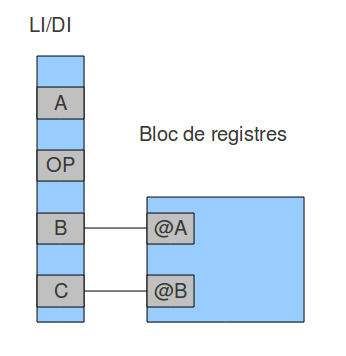
\includegraphics[scale=0.45]{schema-lidi-registres.png}
    \caption{Zoom sur le bloc de registres et le premier étage LI/DI du pipeline}
    \label{schema-lidi-registres}
\end{figure}

Lors d’un tick d'horloge, LI/DI met à jour ses sorties B et C. Le bloc de registres prend aussi en compte lors de ce tick la valeur de ses entrées @A et @B avec le B et C de LI/DI, sauf que ces dernières n’ont pas eu le temps de se mettre en jour quand les entrées @A et @B du bloc de registres capturent leur entrée. Du coup, il fallait un autre tick pour que le bloc de registre prenne en compte les bonnes valeurs. Cela décalait toute la propagation dans le pipeline. Nous avons donc tout mis en asynchrone pour ne laisser que les étages du pipeline calés sur la clock.

\subsection{La gestion des aléas}

La gestion des aléas est difficile, tous les prendre en compte est une tâche ardue. Le problème avec les aléas est de définir le lien entre chaque opération. Par exemple, prenons ces deux instructions : \texttt{COP R0 R1} suivit de \texttt{COP R2 R0}. Après avoir chargé les instructions dans le pipeline, la première instruction se trouve dans le registre DI/EX et la deuxième dans LI/DI. À cette étape-là, on a chargé les valeurs des registres \texttt{R0} et \texttt{R1} mais l'opération ne prendra effet sur les registres qu'après passage de l'étage MEM/ER. On voit bien dans ce cas que la prochaine opération, si on ne gère pas l'aléa, récupèrera la vieille valeur de \texttt{R0} qui était censée être écrasée à l'opération précédente. Il va falloir donc générer une bulle (injection de \texttt{NOP}) en attendant que l'instruction précédente ait affecté le registre \texttt{R0}. On peut trouver des aléas dans beaucoup de cas (opérations arithmétiques, saut, \ldots), c'est pourquoi il est difficile d'être exhaustif. Le plus sûr moyen de les éviter serait de créer des bulles à chaque opération mais alors le pipeline n'aurait plus aucun intérêt.\\

Notre processeur gère bien les aléas liés à chaque opération. On pouvait distinguer deux familles :
\begin{itemize}
\item{ceux liés aux registres}
\item{ceux liés aux sauts inconditionnels}
\item{ceux liés aux sauts conditionnels}
\end{itemize}

\vspace{10pt}

On a créé un contrôleur qui se base sur le contenu des quatres registres du pipeline et suivant leurs valeurs va activer une des trois sorties :
\begin{itemize}
\item{sortie \texttt{alea} : on surveille les numéros de registres situé à la partie A de l'instruction car c'est lui qui recevra le résultat de l'opération. Si dans les instructions suivantes, le numéro de registre situé en B ou C est le même, il va falloir attendre que l'opération  atteigne le dernier étage du pipeline pour être traitée. En attendant, on injecte des \texttt{NOP}.}

\item{sortie \texttt{jump\_JMP} : on injecte des \texttt{NOP} à la place des prochaines opérations et on propage notre \texttt{JMP} jusqu'à la sortie de l'ALU où on va récupérer la nouvelle valeur de l'IP (\textit{Instruction Pointer}) et lui affecter. Ce n'est qu'après affectation de cette valeur que l'on va pouvoir reprendre le \textit{fetch} des opérations.}

\item{sortie \texttt{jump\_JMF} : on injecte des \texttt{NOP} à la place des prochaines opérations et on propage notre \texttt{JMF} jusqu'à la sortie de l'ALU. La valeur du registre de condition récupérée à  l'étage DI/EX stocke le résultat de la condition booléenne. Suivant cette valeur (1 pour \texttt{true}, 0 pour \texttt{false}), soit on arrête d'injecter des \texttt{NOP} et on continue le cycle normal, soit on saute à l'adresse récupérée en sortie de l'ALU (cette adresse doit être calculée car le décalage est relatif donc nécessite un calcul par rapport à la position courante).}
\end{itemize}

\vspace{10pt}

Voici un extrait du code du contrôleur d'aléas :
\begin{lstlisting}[language=VHDL]
  --------------------------------------------------------------
  -- GESTION DES ALEAS
  --------------------------------------------------------------
  alea <= '1' when (	(
  -- gestion de la copie et du store
  (LIDI(INDEX_OP) = COP or LIDI(INDEX_OP) = STORE)
  and (
  (LIDI(INDEX_B) = DIEX(INDEX_A) and DIEX(INDEX_OP) /= NOP) or
  (LIDI(INDEX_B) = EXMem(INDEX_A) and EXMem(INDEX_OP) /= NOP))
  ) or (
  -- gestion des operations arithmetiques
  (LIDI(INDEX_OP) = ADD
  or LIDI(INDEX_OP) = MUL
  or LIDI(INDEX_OP) = DIV
  or LIDI(INDEX_OP) = SUB
  or LIDI(INDEX_OP) = INF 
  or LIDI(INDEX_OP) = SUP
  or LIDI(INDEX_OP) = EQU )
  and (
  (LIDI(INDEX_B) = DIEX(INDEX_A) and DIEX(INDEX_OP) /= NOP) or
  (LIDI(INDEX_B) = EXMem(INDEX_A) and EXMem(INDEX_OP) /= NOP) or
  (LIDI(INDEX_C) = DIEX(INDEX_A) and DIEX(INDEX_OP) /= NOP) or
  (LIDI(INDEX_C) = EXMem(INDEX_A) and EXMem(INDEX_OP) /= NOP)
  )
  )
  )
  else '0';
  
  jump_JMP <= '1' when ( (LIDI(INDEX_OP) = JMP and DIEX(INDEX_OP) /= NOP) or DIEX(INDEX_OP) = JMP or EXMem(INDEX_OP) = JMP )
  else '0';
  
  jump_JMF <= '1' when (LIDI(INDEX_OP) = JMF and DIEX(INDEX_OP) /= NOP) or DIEX(INDEX_OP) = JMF or EXMem(INDEX_OP) = JMF
  else '0';
\end{lstlisting}

Lorsqu'on a récupéré le résultat du contrôleur d'aléas et qu'une des trois sorties est activée, il faut d'abord décrémenter le PC. Ceci nous permet de retourner à l'adresse de l'instruction précédente pour pouvoir la recharger lorsque l'aléa sera terminé. On bloque ensuite l'incrémentation du PC jusqu'à disparition de l'aléa.